\documentclass[12pt]{article}
%%%%%%%%%%%%%%%%
% Packages
%%%%%%%%%%%%%%%%

\usepackage[top=1cm,bottom=1.1cm,left=1.25cm,right= 1.25cm]{geometry}
\usepackage[parfill]{parskip}
\usepackage{graphicx, fontspec, xcolor,multicol, enumitem, setspace, amsmath, changepage}
\DeclareGraphicsRule{.tif}{png}{.png}{`convert #1 `dirname #1`/`basename #1 .tif`.png}

%%%%%%%%%%%%%%%%
% User defined colors
%%%%%%%%%%%%%%%%

% Pantone 2015 Fall colors
% http://iwork3.us/2015/02/18/pantone-2015-fall-fashion-report/
% update each semester or year

\xdefinecolor{custom_blue}{rgb}{0, 0.32, 0.48} % FROM SPRING 2016 COLOR PREVIEW
\xdefinecolor{custom_darkBlue}{rgb}{0.20, 0.20, 0.39} % Reflecting Pond  
\xdefinecolor{custom_orange}{rgb}{0.96, 0.57, 0.42} % Cadmium Orange
\xdefinecolor{custom_green}{rgb}{0, 0.47, 0.52} % Biscay Bay
\xdefinecolor{custom_red}{rgb}{0.58, 0.32, 0.32} % Marsala

\xdefinecolor{custom_lightGray}{rgb}{0.78, 0.80, 0.80} % Glacier Gray
\xdefinecolor{custom_darkGray}{rgb}{0.35, 0.39, 0.43} % Stormy Weather

%%%%%%%%%%%%%%%%
% Color text commands
%%%%%%%%%%%%%%%%

%orange
\newcommand{\orange}[1]{\textit{\textcolor{custom_orange}{#1}}}

% yellow
\newcommand{\yellow}[1]{\textit{\textcolor{yellow}{#1}}}

% blue
\newcommand{\blue}[1]{\textit{\textcolor{blue}{#1}}}

% green
\newcommand{\green}[1]{\textit{\textcolor{custom_green}{#1}}}

% red
\newcommand{\red}[1]{\textit{\textcolor{custom_red}{#1}}}

%%%%%%%%%%%%%%%%
% Coloring titles, links, etc.
%%%%%%%%%%%%%%%%

\usepackage{titlesec}
\titleformat{\section}
{\color{custom_blue}\normalfont\Large\bfseries}
{\color{custom_blue}\thesection}{1em}{}
\titleformat{\subsection}
{\color{custom_blue}\normalfont}
{\color{custom_blue}\thesubsection}{1em}{}

\newcommand{\ttl}[1]{ \textsc{{\LARGE \textbf{{\color{custom_blue} #1} } }}}

\newcommand{\tl}[1]{ \textsc{{\large \textbf{{\color{custom_blue} #1} } }}}

\usepackage[colorlinks=false,pdfborder={0 0 0},urlcolor= custom_orange,colorlinks=true,linkcolor= custom_orange, citecolor= custom_orange,backref=true]{hyperref}

%%%%%%%%%%%%%%%%
% Instructions box
%%%%%%%%%%%%%%%%

\newcommand{\inst}[1]{
\colorbox{custom_blue!20!white!50}{\parbox{\textwidth}{
	\vskip10pt
	\leftskip10pt \rightskip10pt
	#1
	\vskip10pt
}}
\vskip10pt
}

%%%%%%%%%%%
% App Ex number    %
%%%%%%%%%%%

% DON'T FORGET TO UPDATE

\newcommand{\appno}[1]
{4.3}

%%%%%%%%%%%%%%
% Turn on/off solutions       %
%%%%%%%%%%%%%%

% Off
\newcommand{\soln}[2]{$\:$\\ \vspace{#1}}{}

%%% On
%\newcommand{\soln}[2]{\textit{\textcolor{custom_red}{#2}}}{}

%%%%%%%%%%%%%%%%
% Document
%%%%%%%%%%%%%%%%

\begin{document}
\fontspec[Ligatures=TeX]{Helvetica Neue Light}

Dr. \c{C}etinkaya-Rundel \hfill Sta 101: Data Analysis and Statistical Inference \\
Duke University - Department of Statistical Science \hfill \\

\ttl{Application exercise \appno{}: \\
Power}

\inst{$\:$ \\
Team name: \rule{10cm}{0.5pt} \\
$\:$ \\
Lab section: $\qquad$ 8:30 $\qquad$ 10:05 $\qquad$ 11:45 $\qquad$ 1:25 $\qquad$ 3:05 \\
$\:$ \\
Write your responses in the spaces provided below. WRITE LEGIBLY and SHOW ALL WORK! 
Only one submission per team is required. One team will be randomly selected and their 
responses will be discussed and graded. Concise and coherent are best!}

%%%%%%%%%%%%%%%%%%%%%%%%%%%%%%%%%%%%

 In a study of the periodical cicada (\textit{Magicicada septendecim}), researchers measured the hind tibia lengths of the shed skins of 110 individuals. Results for males and females are shown in the accompanying table.

\begin{center}
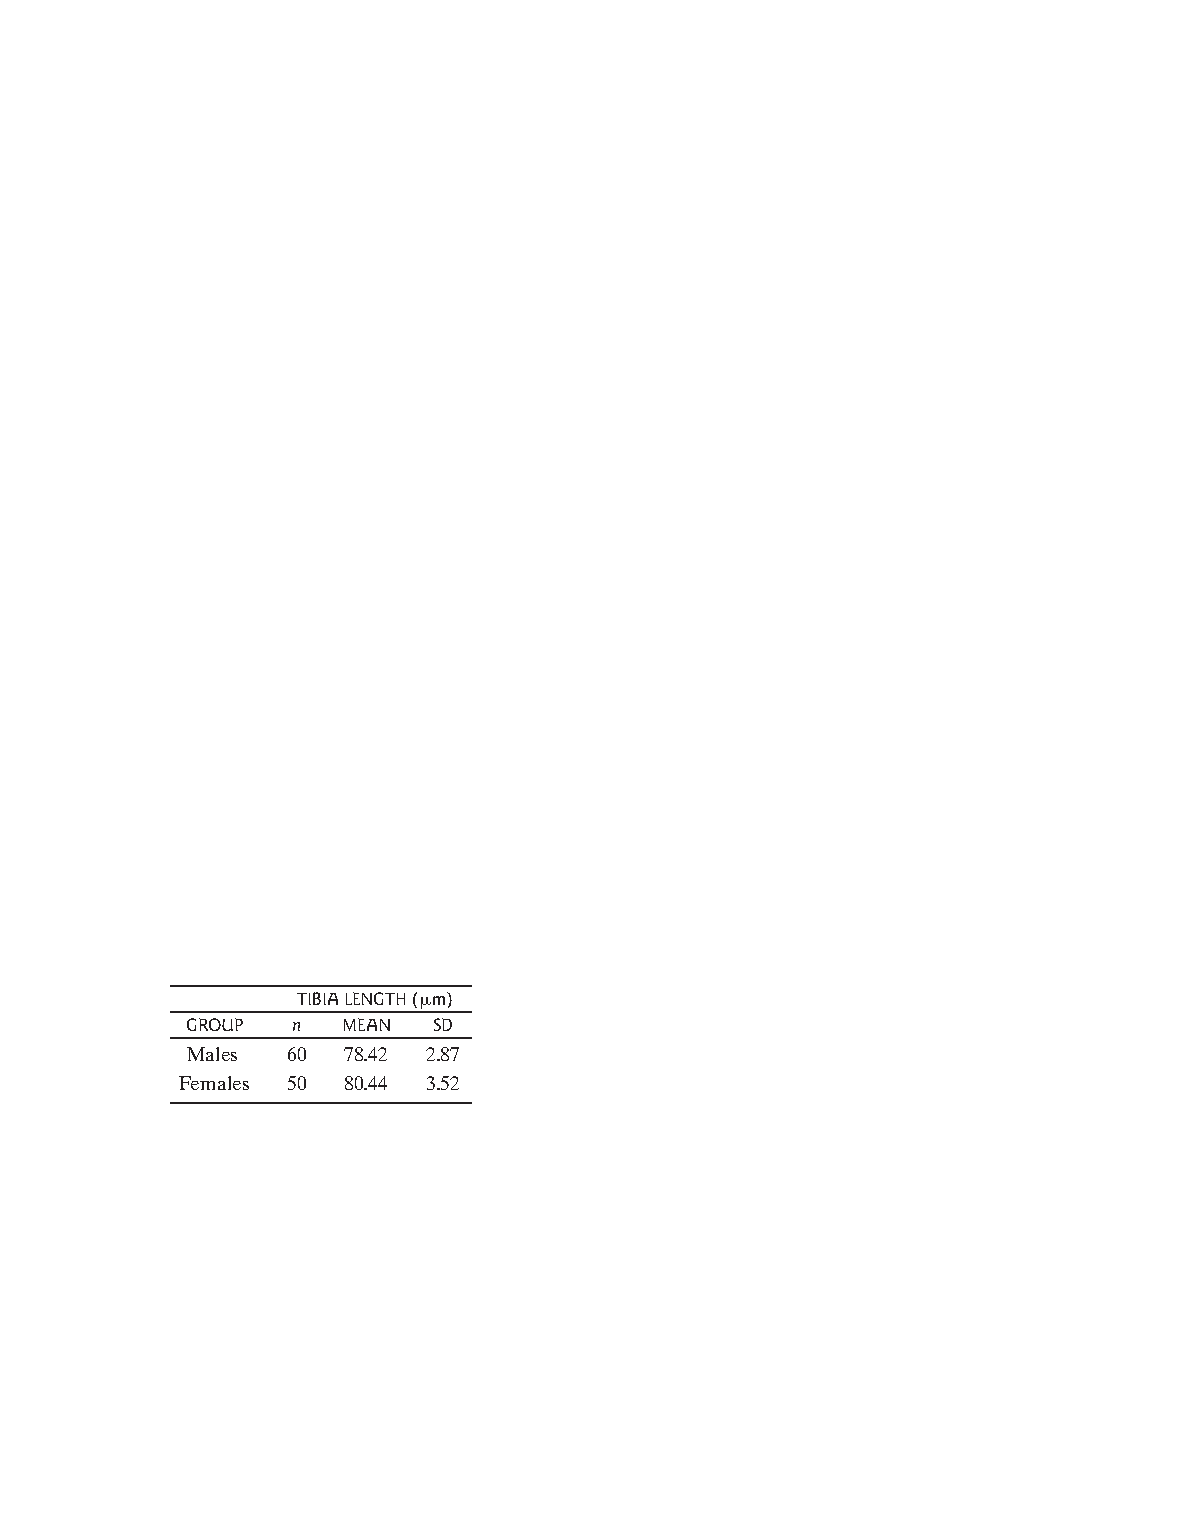
\includegraphics[width=0.3\textwidth]{7_2_8.pdf}
\end{center}

We want to test to see if there is a difference between the average tibia length of male and female cicadas.
Calculate the power of the test to detect a difference 2 $\mu$m. 
 
\soln{7cm}{$H_0$ and $H_A$ are as is part (a).\\
$SE = \sqrt{\frac{2.87^2}{6}+\frac{3.52^2}{5}} = 1.962$\\
\\
$T = (78.42 - 80.44)/1.962 = -1.03$, $df = \text{min}(6-1,5-1) = 4$\\
$\text{P-value} = P(T<-1.03)+P(T>1.03) = 0.3612$\\
We fail to reject $H_0$.\\
\item Step 0: 
\[ H_0: \mu_1 = \mu_2, \quad H_A: \mu_1 \ne \mu_2, \quad \alpha = 0.05, \quad SE = 0.62, \quad \delta=2, \quad n_1=60, \quad n_2=50 \]
Step 1: 
\begin{align*}
P\left(T > \frac{\bar{x}_1-\bar{x}_2 - 0}{0.62} \text{ or } T < \frac{\bar{x}_1-\bar{x}_2 - 0}{0.62} \right) \leq 0.05 \\
\frac{\bar{x}_1-\bar{x}_2 - 0}{0.62} > 2.01 \text{ or } \frac{\bar{x}_1-\bar{x}_2 - 0}{0.62} < -2.01 \\
\bar{x}_1-\bar{x}_2 > 1.246 \text{ or } \bar{x}_1-\bar{x}_2 < -1.246 
\end{align*}
Step 2: Assume $\frac{\bar{x}_1-\bar{x}_2 - \delta}{SE} \sim T_{df=49}$,
\begin{align*}
&P(\bar{x}_1-\bar{x}_2 > 1.246 \text{ or } \bar{x}_1-\bar{x}_2 < -1.246) \\
&= P(T > (1.246-2)/0.62 \text{ or } T < (-1.246-2)/0.62) \\
&= P(T > -1.216) + P(T < -5.235) = 0.8851 + 0.0000 = 0.8851 
\end{align*}
}

%%%%%%%%%%%%%%%%%%%%%%%%%%%%%%%%%%%%

\end{document}